\subsection{Naive Bayes Optimization}
\textbf{LAPLACE}

To find one of the the best settings for the Naive Bayes, a contour for the number of bins and the accumulated variance in the PCA analysis was made.

\begin{figure}[H]
\centering
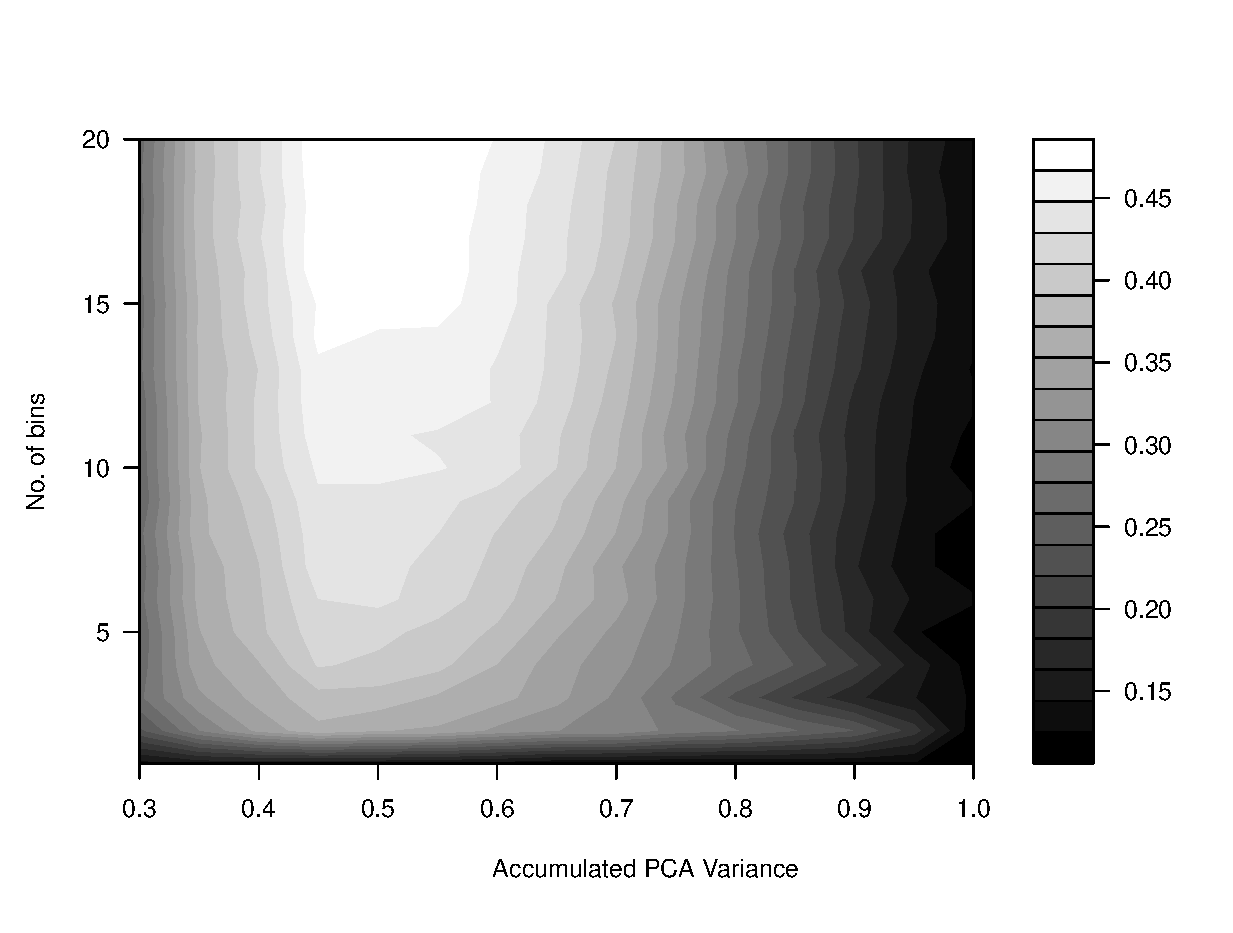
\includegraphics[width = \textwidth]{graphics/contour_bins_vs_pca}
\caption{Contour of the success rate of the Naive Bayes with accumulated PCA going from 0.3 to 1 and the number of bins from 2 to 192.
The data was normalized using z-score first and the Laplace value was set to 1.
The contour was created with G3M2 data in the test set and the remaining 15 loadable datasets in the training set.}
\label{fig:contour_bin-vs-pca}
\end{figure}

From figure \ref{fig:contour_bin-vs-pca} it can be seen that the best point goes out of the view, and is in fact increasing, indicating that it gets better the higher dimensional the data is. The best bin size can hence not be determined. The most optimum point would be around 40 bins and an accumulative PCA of 50\% as at this point, the increase PCA and bins does not improve the success by an considerably enough compared to how much the timing would increase.
These values for bins, PCA and Laplace are then used to compare all people with the rest of the class in figure \ref{fig:comp_naiveBayes}.

\begin{figure}[H]
\centering
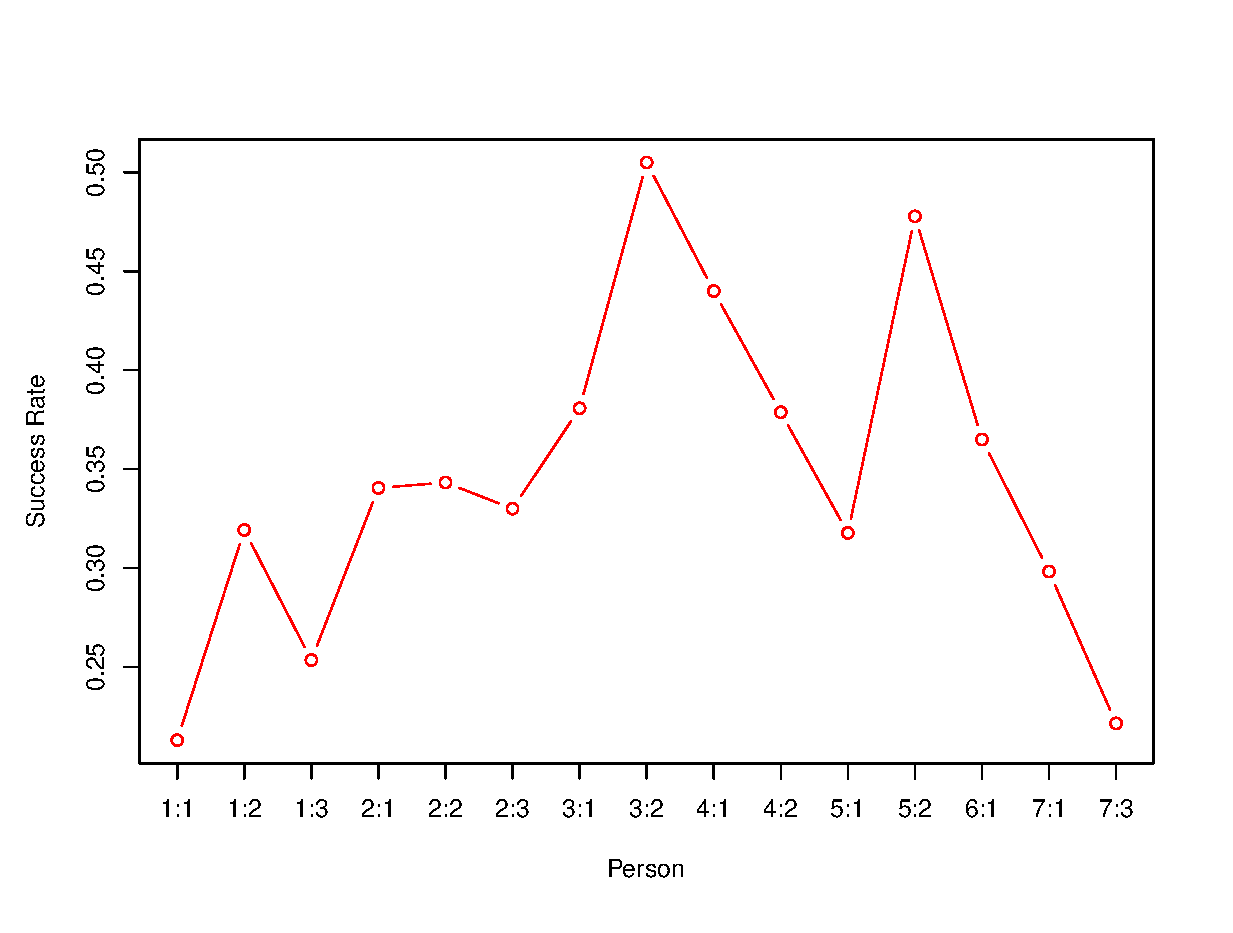
\includegraphics[width = \textwidth]{graphics/graph_baye_comparison}
\caption{Comparison of Naive Bayes for one person with the rest of the class.
Where bins is 40, PCA is 50\% and laplace of 1. The mean success rate is XX.X\%.}
\label{fig:comp_naiveBayes}
\end{figure}

The timing was measured with different bin sizes. 
In figure \ref{fig:baye_timing} the timing and success can be seen.
The timing is linear and there is no increase in successful classifications with more than 100 bins. 
The timing doesn't include the time it took to 

\begin{figure}
\centering
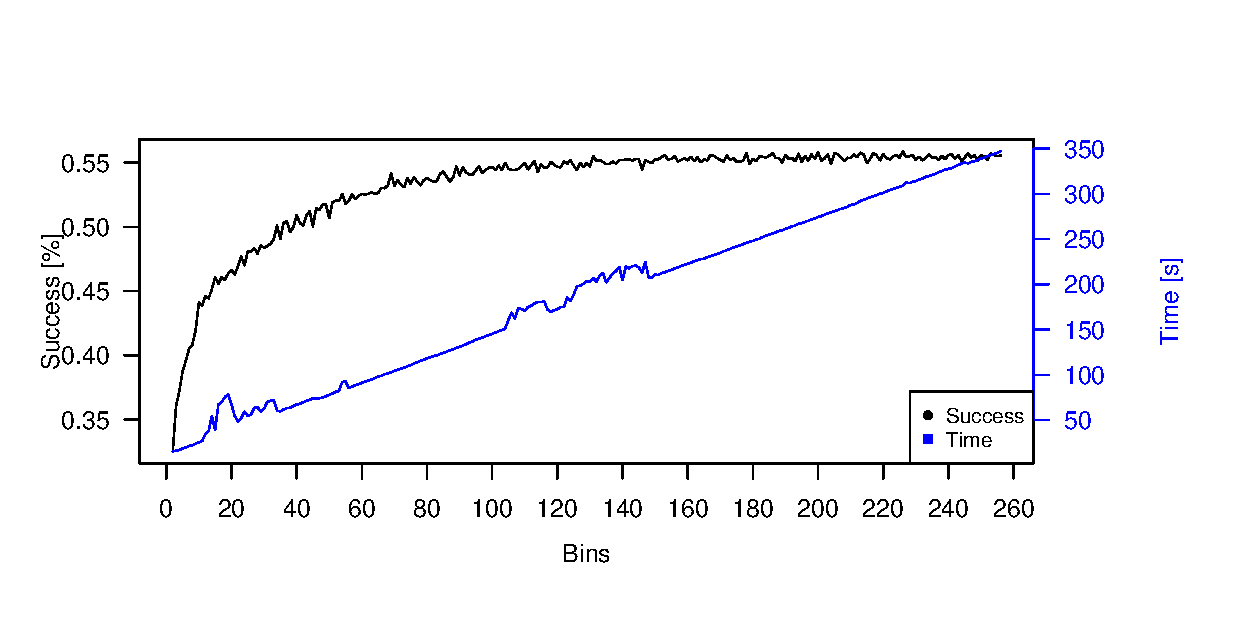
\includegraphics[width = \textwidth]{graphics/baye_timing_bins}
\caption[Timing with different bin sizes]{Timing and success of different bin sizes. Data was tested on Group 3 member 2's data vs 16 people.}
\label{fig:baye_timing}
\end{figure}
